%!TEX root = ./icml2016.tex
\section{Experiments}

\subsection{Synthetic data}
\begin{figure}[t]
	\centering
	
	\subfigure[E=5, K=5, D=5\label{fig:syn1}]{
	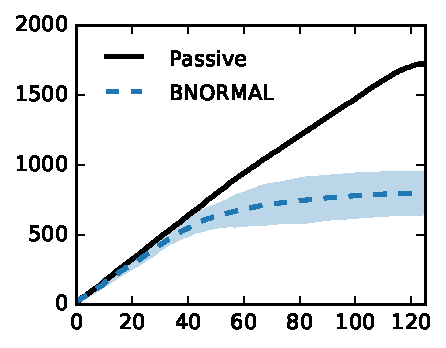
\includegraphics[width=0.42\linewidth]{images/toy_5_5_5.pdf}
	}
	\subfigure[E=10, K=10, D=5\label{fig:syn2}]{
	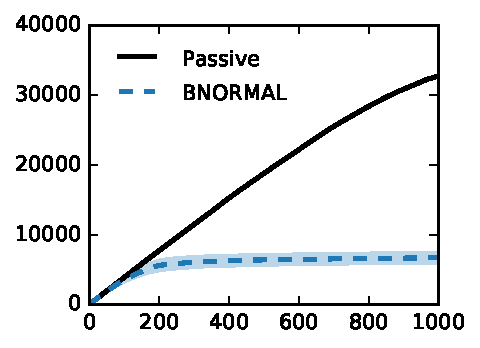
\includegraphics[width=0.45\linewidth]{images/toy_10_10_5.pdf}				
	}
%	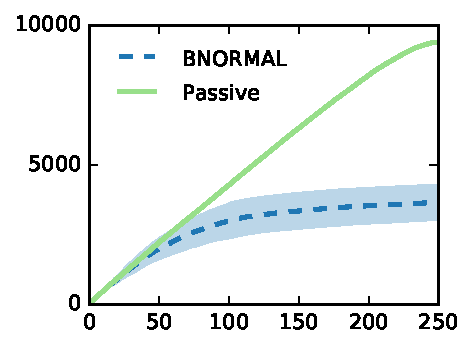
\includegraphics[width=0.32\linewidth]{images/toy_5_10_5.pdf}			
%	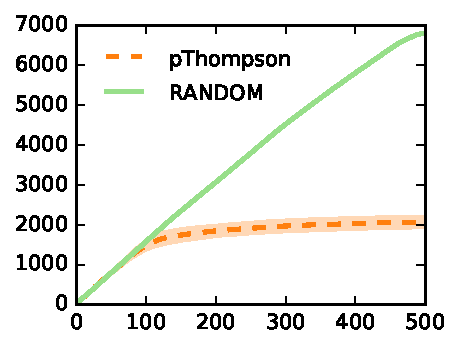
\includegraphics[width=0.32\linewidth]{images/toy_10_5_5.pdf}				
	\caption{\label{fig:synthetic} Cumulative regret of particle Thompson sampling on different sizes of the synthetic dataset. E, K, and D denote the number of entities, relations, and latent dimensions, respectively. The synthetic dataset is generated by the model assumption. We compared the particle Thompson sampling with passive sampling method. The averaged cumulative regrets are plotted with one standard error. As the model obtained more and more labeled samples from Thompson sampling, the cumulative regrets are converged. }
\end{figure}

To verify the particle Thompson sampling, we first synthesize data based on the model assumptions and run the Thompson sampling algorithm. By following the model assumptions in Eq. \ref{eqn:entity_gen} to \ref{eqn:triple_gen}, we randomly generate triples based on randomly sampled entities and relations. Every entities and relations are generated from zero-mean isotropic multivariate normal distribution, where we set the variance parameters $\sigma_e$, $\sigma_r$, and $\sigma_x$ to 10, 10, and 0.1, respectively.

To measure the performance on synthetic dataset, we compute the cumulative regret of proposed algorithm at each time $n$ as follows:
\begin{align}
R(n) = \sum_{t=1}^{n} x_t - x^{*}_t,
\end{align}
where $x^*_t$ is the highest triple among triples that have not been chosen up to time $t$. Unlike the general Bandit setting where one can select a single item multiple times, in our formulation, we can select one triple only once. So after selecting a triple at time $t$, the selected triple will be removed from a set of candidate triples.

Figure \ref{fig:synthetic} shows the cumulative regret of the algorithm on the synthetic data with varying size of entities and relations. We compare the cumulative regret of the particle Thompson sampling with the passive learning method where the model choose a random triple at each time. All results are averaged over 10 individual runs with different initializations. For every experiment, the cumulative regret of the Thompson sampling method was bounded after a certain number of interactions whereas the cumulative regret of passive learning increases linearly. This result indicates the particle sampling correctly inferred latent features of entities and relations as the interaction increases.

\subsection{particle Thompson sampling}
\begin{table}[t]
\centering
\caption{\label{tbl:dataset}Description of datasets.}
\begin{tabular}{l | r | r | r | r}
Dataset &  \# rel & \# entities & \# triples & sparsity \\ \hline
Kinship & 26 & 104  & 10,790 & 0.038 \\
UMLS & 49 &135  & 6,752 & 0.008 \\
Nation & 56 & 14  & 2,024 & 0.184 \\
%Wordnet & 11 & 38,696  &123,429 & 7.5e-06\\
%Wordnet(N) & 10 & 836 & 1,766 & 2.5e-04\\
\end{tabular}
\end{table}

\begin{figure}[t]
	\centering
	
	\subfigure[KINSHIP]{
	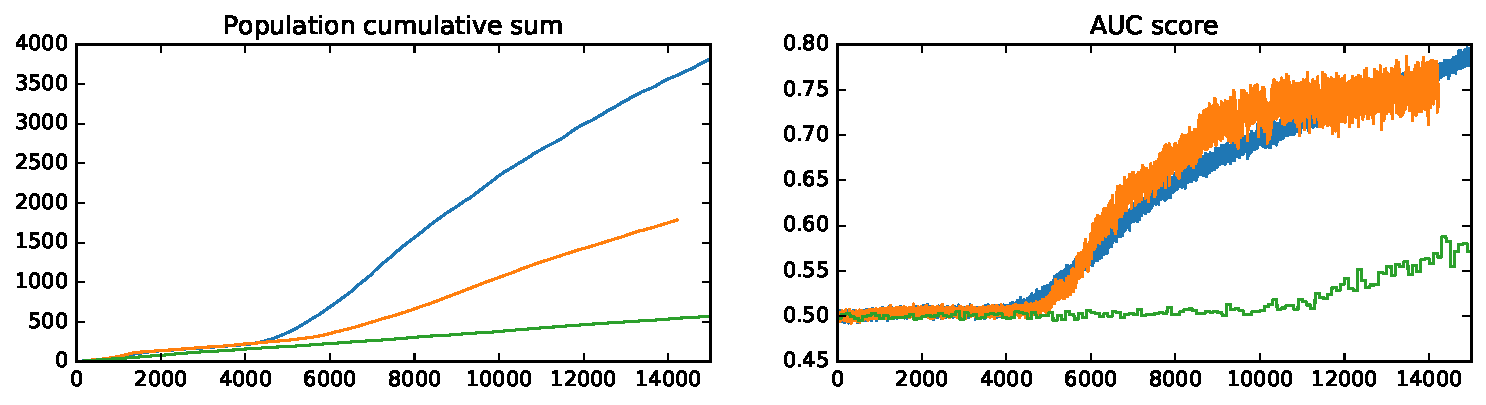
\includegraphics[width=\linewidth]{images/thompson_kinship.pdf}
	}
	\subfigure[UMLS]{
	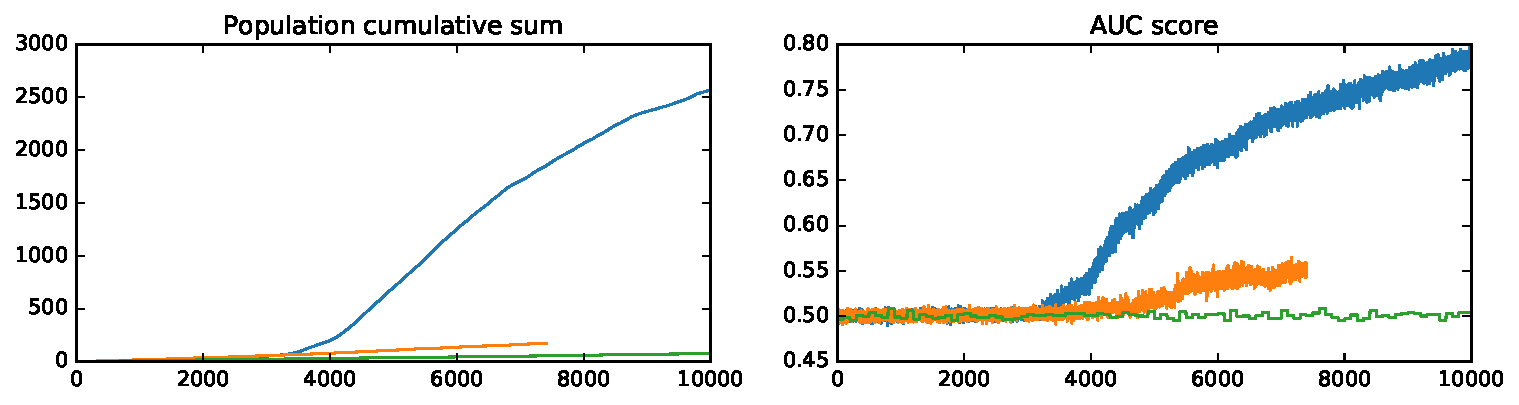
\includegraphics[width=\linewidth]{images/thompson_umls.pdf}				
	}
	\subfigure[NATION]{
	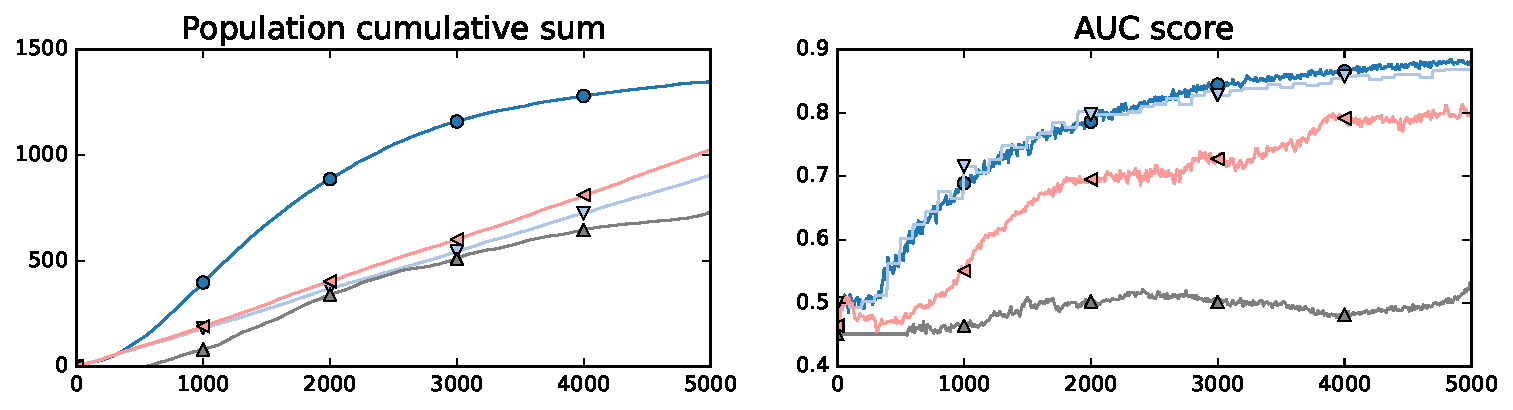
\includegraphics[width=\linewidth]{images/thompson_nation.pdf}				
	}	
	\caption{Placeholder for the future results. Will include the cumulative gain and ROC-AUC score of the developed models with the active and passive learning methods. We will see how the compositional model performs to compare with other models without any initial observation (May include the IBM model without any initial observation).}
\end{figure}

\subsection{Compositional ...}
\begin{figure}[t]
	\centering
	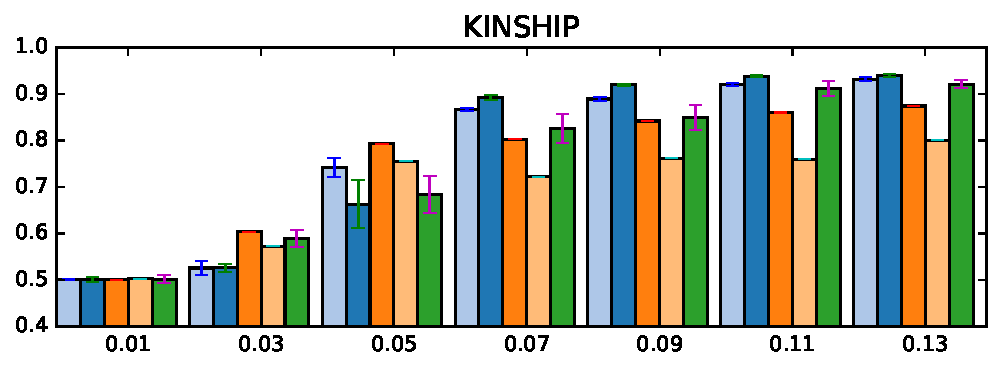
\includegraphics[width=\linewidth]{images/comp_training_error_kinship_small.pdf}
	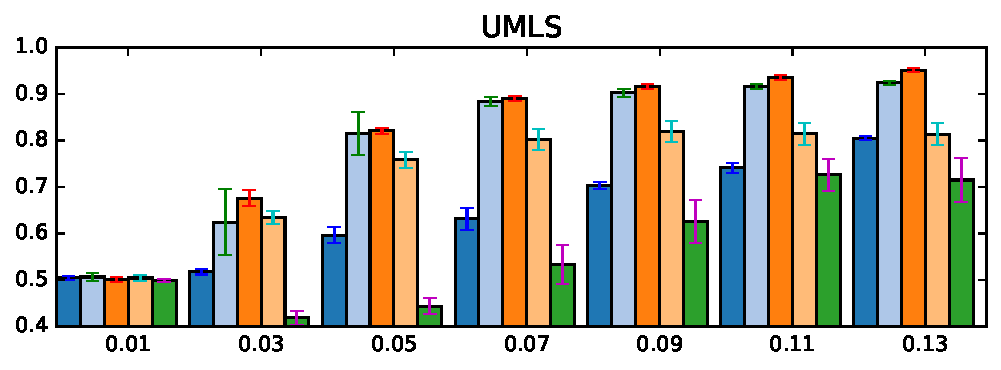
\includegraphics[width=\linewidth]{images/comp_training_error_umls_small.pdf}			
	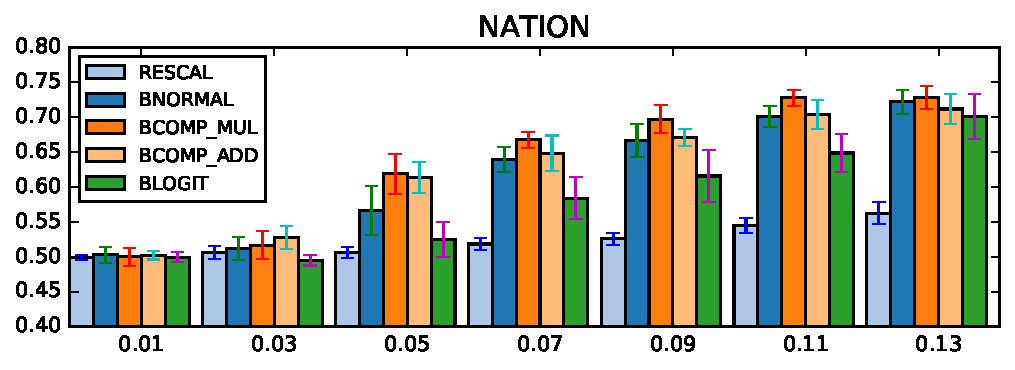
\includegraphics[width=\linewidth]{images/comp_training_error_nation_small.pdf}				
	\caption{\label{fig:r_vs_br} ROC-AUC scores of compositional models. The x-axis denotes the proportion of an observed triples including negative triples used for training models. We  use another 30\% of triples to evaluate the ROC-AUC score. In general, compositional models outperform BRESCAL and BLOGIT model when the size of training set is relatively small, whereas BRESCAL and BLOGIT perform slightly better than or comparable to the compositional models when the size of training set is relatively large. For UMLS dataset, the multiplicative compositional model consistently outperforms the other models across all training proportions.}
\end{figure} 

